\chapter{Containers}\label{cont}

\begin{epigraphs}
\qitem{
La intención de la neolengua no era solamente proveer un medio de expresión a la cosmovisión y hábitos mentales propios de los devotos del Ingsoc, sino también imposibilitar otras formas de pensamiento. Lo que se pretendía era que una vez la neolengua fuera adoptada de una vez por todas y la vieja lengua olvidada, cualquier pensamiento herético, es decir, un pensamiento divergente de los principios del Ingsoc, fuera literalmente impensable, o por lo menos en tanto que el pensamiento depende de las palabras.}{1984\\ George Orwell}
\end{epigraphs}


Los containers~\cite{abbott:2003,alti:2005}, así como muchas otras construcciones matemáticas abstractas, tienen la particularidad de poder ser pensados desde diferentes puntos de vista. Podemos ponernos nuestros {\it lentes de teoría de tipos} o nuestros {\it lentes de teoría de categorías} y visualizar cada construcción en marcos diferentes. En cada caso, lo que cambiará será fundamentalmente el lenguaje en el que se presentan los conceptos y necesariamente, la relación con el mundo teórico que los rodea, los precede y explica.

En este capítulo trataremos de presentar a los containers como una forma particular de representar ciertos tipos paramétricos. Para comenzar, utilizaremos nuestros {\it lentes Agda} de programador funcional-dependiente. La elección de este recurso implica optar por un punto de vista {\it más concreto} (a.k.a. menos abstracto que la visión categórica) y por lo tanto a priori más didáctico, pero sin perder el nivel de correctitud. Correctitud obtenida gracias a las garantías que nos provee un lenguaje-de-programación/demostrador-de-teoremas como lo es Agda.

El universo de containers resulta muy apropiado a la hora de programar genéricamente~\cite{alti:2007} y cobra relevancia al momento de poder representar constructores de tipos funtoriales, en particular, los generadores de los tipos estrictamente positivos. El universo de morfismos de containers, por su parte, tiene el poder expresivo para representar un subconjunto muy interesante de funciones: las que definen transformaciones naturales.

Comenzaremos la exposición, sin embargo, con un ejemplo en lenguaje coloquial, con la intención de presentar la idea de la forma más intuitiva posible. Para continuar, definiremos formalmente los conceptos de container y de extensión y ejemplificaremos su potencialidad, a partir de expresar en estos nuevos términos algunos exponentes ilustres de tipos paramétricos. Luego analizaremos la manera de expresar funciones entre tipos paramétricos, definiendo los morfismos de containers.

Finalmente, cambiaremos el punto de vista, y expresaremos la forma en la que los containers constituyen una categoría, formalizando en Agda la categoría $\Cont$. 


\newpage
\section{Motivación}
\label{sec:containers.motivacion}

Los tipos de datos que nos interesa modelar son aquellos que contienen valores de otros tipos de datos. Como por ejemplo, las listas, los árboles, los streams. Decimos que son tipos de datos parametrizados por otro tipo de datos, el tipo de los valores que almacenan.
Les llamaremos también {\it constructores de tipos} porque construyen un nuevo tipo a partir de otro dado.
No obstante el tipo de los valores que se almacenan es tomado como parámetro por el constructor, la estructura de este último no depende del primero.

Enfoquémonos por ejemplo en el tipo de las listas, definido en Agda de forma inductiva:

\begin{agdacode}
  \label{list}
Listas
  
  \ExecuteMetaData[latex/Aux.tex]{list}
\end{agdacode}
El elemento \AgdaInductiveConstructor{nil} es un habitante de \AgdaDatatype{List} \AgdaBound{X}, para todo \AgdaBound{X} dado y representa la lista vacía.
De forma similar, \AgdaInductiveConstructor{cons} construye una lista agregando un elemento de \AgdaBound{X} a una lista ya dada de elementos de \AgdaBound{X}.
A pesar de no conocer nada sobre el tipo \AgdaBound{X}, podemos definir \AgdaDatatype{List} \AgdaBound{X}, indicio de que la esencia de \AgdaDatatype{List} es independiente de cualquier particularidad de \AgdaBound{X}.
Vemos aquí presente una potencial capacidad de segregar estructura de contenido. Es este potencial el que explotaremos para presentar una forma alternativa de representación.

Es posible pensar a ciertos tipos de datos como un esqueleto, un contenedor, a llenar con datos. 
Las listas como esqueletos se pueden expresar visualmente de la siguiente forma:
\begin{figure}[H]
$$ [] \quad [\bigcirc] \quad [\bigcirc , \bigcirc] \quad [\bigcirc , \bigcirc, \bigcirc] \quad [\bigcirc , \bigcirc, \bigcirc, \bigcirc ] \quad \mbox{ etc.}$$
\caption{Containers de lista}
\label{fig:cList}
\end{figure}

Llamaremos {\it containers} a estos esqueletos. Para dar una lista como un container, proveemos dos coordenadas: por un lado la {\it forma} que tiene el container, y para cada forma, un conjunto de {\it posiciones}.

Si observamos la figura \ref{fig:cList}, advertimos que el conjunto de los números naturales representan de forma unívoca a cada forma de lista: la forma de una lista es su longitud.
Fijada una forma $n$, cada $\bigcirc$ representa un {\it agujero} destinado a ser llenado con datos. Es decir, una posición.
El conjunto de posiciones posibles será el de los números naturales entre $0$ y $n - 1$. Por ejemplo, para el caso de una lista de longitud tres tenemos:
$$[\bigcirc_0 , \bigcirc_1, \bigcirc_2]$$
donde los subíndices identifican las posiciones en la lista.

Al conjunto de naturales menores a $n$ lo definimos como un nuevo tipo de datos \AgdaDatatype{Fin}, indexado en $n$.

\ExecuteMetaData[latex/Aux.tex]{fin}

Notar que \AgdaDatatype{Fin} \AgdaNumber{0} es el tipo vacío, ya que no tenemos ningún constructor que lo habite. Por otra parte, \AgdaDatatype{Fin} ($n$ \AgdaFunction{+} \AgdaNumber{1}) tiene tantos elementos como \AgdaDatatype{Fin} $n$, gracias al constructor \AgdaInductiveConstructor{suc} y uno más, el elemento \AgdaInductiveConstructor{zero}. 
En conclusión, \AgdaDatatype{Fin} $n$ tiene $n$ elementos. Coloquialmente decimos: \AgdaDatatype{Fin} $n$ = $\{0, \ldots, n-1 \}$.


Finalmente, nos queda pendiente proveer un mecanismo para ``llenar'' un esqueleto de lista. Para ello, fijada una forma de lista, nos basta con una función de posiciones en valores.
Por ejemplo, para la lista $[x_1,x_2,x_3]$ de tipo $X$, necesitamos una función que asigne a cada posición, los valores correspondientes de $X$, como muestra la figura \ref{fig:List}:

\begin{figure}[H]
\begin{center}
  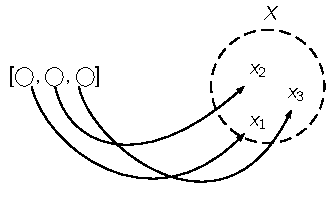
\includegraphics{img/container.pdf}
\end{center}
\caption{Llenando un container de lista}
\label{fig:List}
\end{figure}

Generalizando, llenar un container con valores de un tipo \AgdaBound{X}, es proveer una función que asigne valores de \AgdaBound{X} a cada posición, para cada forma. Llamaremos a esta función, la {\it extensión} del container.
 

\section{Definición y extensión}

A continuación expondremos formalmente esta nueva forma de representación. Para dar una instancia de un nuevo constructor de tipo proveeremos por un lado su estructura en la forma de un {\it container}. Luego, para permitir ``llenar'' al container con datos de tipo \AgdaBound{X}, calcularemos su {\it extensión}. 

%%%%%%%%%%%%%%%%%%%%%%%%%%%%%%%%%%%%%%%%%%%%%%%%
%%     DEFINICION    
%%%%%%%%%%%%%%%%%%%%%%%%%%%%%%%%%%%%%%%%%%%%%%%%

\subsection{Definición}

\begin{definition}
  Un {\it container} es un par ({\it Sh}, {\it Pos}) que notamos \agdaCont{Sh}{Pos} donde

  \begin{itemize}
  \item {\it Sh} es un conjunto de {\it formas} (o {\it shapes} en inglés).
  \item {\it Pos} es es un conjunto de posiciones, para cada forma $s$ en $Sh$. 
      Es decir, es una familia de posiciones indexada por las formas.
  \end{itemize}
\end{definition}


En Agda definimos: 

\begin{agdacode}\label{code:cont}{\it Containers}

\ExecuteMetaData[latex/Container.tex]{cont}
\end{agdacode}

Recordemos que en Agda un record es una tupla donde se le asigna nombre a cada componente y, opcionalmente, un constructor de instancias. Los nombres asignados a cada componente hacen a su vez las veces de destructores del record.
En el caso de \AgdaDatatype{Cont}, construimos sus instancias llamando a  \AgdaInductiveConstructor{$\_\tri\_$} con un \AgdaBound{S} : \AgdaDatatype{Set} y un \AgdaBound{P} : \AgdaBound{S} $\to$ \AgdaDatatype{Set}. Notar que el tipo de los componentes de un record puede depender de componentes anteriores.

Los nombres de campos \Sh y \Pos del record \AgdaDatatype{Cont} definen funciones de destrucción, con tipos:

\sangrar
\Sh : \AgdaDatatype{Cont} $\to$ \AgdaDatatype{Set}

\sangrar
\Pos : (C : \AgdaDatatype{Cont}) $\to$ \Sh C $\to$ \AgdaDatatype{Set}\\
de forma tal que para todo C : \AgdaDatatype{Cont} siempre valga la siguiente igualdad definicional: \Sh C \AgdaInductiveConstructor{$\tri$} \Pos C = C .

\begin{example}
Volviendo al ejemplo de la sección \ref{sec:containers.motivacion},
el container que representa a las listas está dado por el elemento \AgdaFunction{cList}, definido como:

 \ExecuteMetaData[latex/Examples.tex]{clist}

Aludiendo a lo expuesto anteriormente, las listas son aquél tipo cuya forma está dada por su longitud. Es decir, el conjunto de todas las formas posibles será el conjunto de los números naturales y el cero. Fijada una longitud \AgdaBound{n}, el conjunto de posiciones será el de todos los enteros entre \AgdaBound{0} y \AgdaBound{n - 1}. Es decir, es el \AgdaBound{n}-ésimo conjunto finitario.
\end{example}

%%%%%%%%%%%%%%%%%%%%%%%%%%%%%%%%%%%%%%%%%%%%%%%%
%%     EXTENSION    
%%%%%%%%%%%%%%%%%%%%%%%%%%%%%%%%%%%%%%%%%%%%%%%%
 
\subsection{Extensión}
  
Hasta ahora hemos expuesto la forma en que el universo sintáctico de
containers representa a ciertos constructores de tipos. Algunas preguntas que caben hacerse son: ¿Qué constructores son posibles de ser representados como containers? En otras palabras, ¿a qué constructores representan los containers? ¿Cómo estar seguros, más allá de la apelación a la intuición, que un container representa a un constructor determinado?

Antes de contestar esas, entre otras cuestiones, trataremos de dar respuesta a una pregunta más elemental y por lo tanto de más sutil respuesta: ¿Qué es un constructor de tipos?
Una idea intuitiva fue ofrecida al comenzar el capítulo: un constructor de tipos construye un tipo a partir de otro dado genéricamente, en forma de parámetro.
Para ejemplificar dicha aseveración, dimos el elemento \AgdaDatatype{List}, en la definición \ref{list}.
Si observamos dicha definición podemos apreciar que el constructor de tipos \AgdaDatatype{List} tiene el siguiente tipo: 

\sangrar
\AgdaDatatype{List} \AgdaSymbol{:} \AgdaDatatype{Set} \AgdaSymbol{$\to$} \AgdaDatatype{Set}

Otro constructor de tipos posible podría ser, por ejemplo, el que construye pares de elementos de dos tipos distintos:

 \ExecuteMetaData[latex/Aux.tex]{pair}
 
Un ejemplo más, es el de las funciones de un tipo arbitrario en sí mismo. Es decir, el tipo de datos \AgdaDatatype{Endo} $X$, expuesto en el siguiente código, engloba a todas las funciones con tipo $X \to X$. 
 
 \ExecuteMetaData[latex/Aux.tex]{endo}

 Tanto el constructor de tipos \AgdaDatatype{Pair}, como el constructor \AgdaDatatype{Endo} no serán posibles de ser representados como containers. Esto se debe a que restringimos el análisis a {\it ciertos} constructores de tipo.
Por simplicidad, el tipo de datos \AgdaDatatype{Pair} no será contemplado, puesto que nos limitamos a constructores de un sólo argumento. Sin embargo, toda la teoría de containers se extiende fácilmente a constructores de más argumentos. En tal caso sí incluiríamos al tipo de los pares. 
 Por otro lado, tampoco podremos representar al tipo \AgdaDatatype{Endo} puesto que nos conciernen aquellos constructores que cumplen ciertas propiedades y a los que llamaremos {\it funtores}.


\begin{definition} \label{def:funtor}
  Un constructor de tipos \AgdaDatatype{F} \AgdaSymbol{:} \AgdaDatatype{Set} \AgdaSymbol{$\to$} \AgdaDatatype{Set} es un {\it funtor}~\cite{plotkin+reynolds} si existe una función de mapeo

 \ExecuteMetaData[latex/Aux.tex]{map}\\
 tal que

 \sangrar
 $
 \left \{ \begin{array}{ll}
 \AgdaFunction{map}\ \AgdaFunction{id} = \AgdaFunction{id} &
 \\ \AgdaFunction{map}\ f \circ \AgdaFunction{map}\ g = \AgdaFunction{map}\ (f\ \AgdaFunction{$\circ$}\ g) & \quad \forall\ f :  Z \to B,\ g : A \to Z
 \end{array}
 \right. 
 $
 
Es decir, un funtor es un constructor \AgdaDatatype{F} que cumple con ciertas propiedades extra. Siempre que exista una función entre los tipos $A$ y $B$ habrá una función entre \AgdaDatatype{F} $A$ y \AgdaDatatype{F} $B$ de forma tal que las identidades y composiciones se preserven. 
 
\end{definition}

\vspace{1ex}

El constructor de pares \AgdaDatatype{Pair}
no será funtor sino hasta que fijemos el tipo de uno de los dos elementos del par. Por ejemplo, fijando el primer tipo al de los naturales se obtiene:

 \ExecuteMetaData[latex/Aux.tex]{pairNX}

En el caso de \AgdaDatatype{Endo} no es posible definir una función \AgdaFunction{map} que cumpla con los requisitos de la definición.
 
\vspace{1ex}

Retomando nuestra exposición, presentaremos a continuación
la noción de {\it extensión} de un container, que hará posible volver a interpretarlos como constructores de tipos en su forma funtorial.

Si \AgdaBound{cF} \AgdaSymbol{:} \AgdaDatatype{Cont} es un container, entonces su extensión, que notamos \agdaExt{\AgdaBound{cF}}, será un funtor:

\sangrar
\agdaExt{\AgdaBound{cF}} \AgdaSymbol{:} \AgdaDatatype{Set} \AgdaSymbol{$\to$} \AgdaDatatype{Set}

Intuitivamente, la extensión permitirá llenar un container con valores del tipo argumento.
En caso en que necesitemos precisión en la exposición, llamaremos {\it funtor container} a un funtor obtenido de calcular la extensión a un container. 

\vspace{2ex}

\begin{definition}
  La {\it extensión} del container \agdaCont{S}{P} sobre el conjunto \AgdaBound{X} es el conjunto de pares $(s, f)$ donde $s \in S$ y $f : Ps \to X$.
  Lo notamos \agdaExt{\agdaCont{S}{P}}.

Dado un caso particular de forma, tenemos un conjunto de posiciones. La extensión requiere de una función de posiciones en valores. 

\begin{agdacode}\label{code:cont:ext}{\it Extensión de containers}

\ExecuteMetaData[latex/Container.tex]{ext}
\end{agdacode}

Dicho de otra forma, \agdaExt{\agdaCont{S}{P}}
define familias de funciones $P s \to X$ de posiciones en valores por cada forma $s$ del conjunto $S$.
\end{definition}

\begin{example}
Entonces, para completar nuestro ejemplo de las listas, podemos finalmente calcular su extensión y así volver al <<mundo real>>. 

\ExecuteMetaData[latex/Examples.tex]{list}

Incluso es posible definir los constructores originales del tipo \AgdaDatatype{List} dado inductivamente:

\ExecuteMetaData[latex/Examples.tex]{listconstructors}

Dado que la forma de una lista es su longitud, el valor 
\AgdaFunction{nil} construye un elemento con forma igual a \AgdaNumber{0}. La función que asigna valores a posiciones es la función vacía, representada en Agda por $(\lambda\; ())$, ya que la forma nula no tiene posiciones.
Por su parte, la función \AgdaFunction{cons} \AgdaBound{x} construye una lista cuya forma es el sucesor de la lista argumento, puesto que \AgdaFunction{cons} aumenta su longitud en uno. Además, ahora la posición \AgdaInductiveConstructor{zero} mapea al nuevo elemento \AgdaBound{x}, desplazando al resto.
\end{example}

  A pesar de haber sostenido que los containers nos proveen una forma de construir funtores recurriendo al cálculo de su extensión, nos queda pendiente evidenciar que esto es cierto. Intuitivamente, si un container es un esqueleto donde se guardarán datos, resulta lógico que los datos almacenados puedan ser modificados sin tocar ese esqueleto que los contiene.
  A continuación definimos la función \AgdaFunction{map} para containers. Queda pendiente demostrar que dicha función cumple con los requerimientos de la definición \ref{def:funtor}

\begin{definition} Sea $f$ una función de $X$ en $Y$ y $C$ un container. Se define el mapeo de $f$ sobre el funtor container \agdaExt{$C$} como una nueva función de \agdaExt{$C$} $X$ en \agdaExt{$C$} $Y$ que preserva las formas y aplica $f$ a los elementos almacenados, como se indica a continuación:

\ExecuteMetaData[latex/Container.tex]{map}
\end{definition}

Así como vemos que la extensión de un container resulta ser un endofuntor en \AgdaDatatype{Set}, y que lógicamente dichos funtores pueden componerse y obtener así otro funtor, también podemos componer containers antes de calcular su extensión. Es decir, los containers son cerrados bajo composición, siendo la extensión de la composición equivalente a la composición de las extensiones.

\begin{definition} Definimos la composición de los containers $C$ y $D$ como el container que tiene por conjunto de formas posibles a \agdaExt{$C$} (\AgdaField{Sh} $D$). Es decir que por cada posición en una forma $c$ de $C$, tenemos una forma de $D$.

  Dada una forma $(c,d)$, siendo $c$ forma de $C$ y $d$ una función de posiciones en $C$ hacia formas en $D$, el conjunto de posiciones es el conjunto de pares dependientes $(p,q)$, donde $p$ es una posición en $C$ en la forma $c$ y $q$ una posición de $D$ en la forma $(d \, p)$.

  \ExecuteMetaData[latex/Composition.tex]{compose}
\end{definition}

Componer constructores de tipos da como resultado constructores en cierta forma {\it anidados}. Con la composición podemos formar, por ejemplo, las listas de árboles o los árboles de listas. En el ejemplo \ref{ex:cont:comp} veremos un ejemplo de su uso.

\vspace{3ex}

En conclusión, hemos expuesto una sintaxis para representar ciertos constructores de tipo funtoriales \AgdaDatatype{F} \AgdaSymbol{:} \AgdaDatatype{Set} \AgdaSymbol{$\to$} \AgdaDatatype{Set} como un container
\AgdaFunction{cF} \AgdaSymbol{:} \AgdaDatatype{Cont}.
La función de extensión se constituye como un mecanismo para obtener nuevamente un funtor, tal que \agdaExt{\AgdaFunction{cF}} $\cong$
\AgdaDatatype{F}.

\subsection{Ejemplos}

%%%%%%%%%%%%%%%%%%%%%%%%%%%%%%%%%%%%%%%%%%%%%%%%
%%     ID
%%%%%%%%%%%%%%%%%%%%%%%%%%%%%%%%%%%%%%%%%%%%%%%%

\begin{example}
  Comencemos con uno de los ejemplos más sencillos que podamos construir: el container que define al tipo identidad.
  Recordemos la definición canónica de \AgdaDatatype{Id}, expresada en Agda:

  \ExecuteMetaData[latex/Aux.tex]{id}
  
  En este caso tenemos una única forma posible, con una única posición.

\begin{center}
\AgdaInductiveConstructor{identity}$\bigcirc$
\end{center}

  El elemento que simbolizará al tipo \AgdaDatatype{Id} en el universo de containers será el siguiente, siendo \AgdaDatatype{$\top$} el conjunto que tiene a \AgdaInductiveConstructor{tt} como único el elemento.

  \ExecuteMetaData[latex/Examples.tex]{cId}

  
  Al extender dicho container, obtenemos un constructor de tipos \AgdaDatatype{Id}. Podemos definir también el constructor de datos \AgdaFunction{identity}.

  \ExecuteMetaData[latex/Examples.tex]{Id}
\end{example}
\vspace{2ex}


%%%%%%%%%%%%%%%%%%%%%%%%%%%%%%%%%%%%%%%%%%%%%%%%
%%     K
%%%%%%%%%%%%%%%%%%%%%%%%%%%%%%%%%%%%%%%%%%%%%%%%

\begin{example} \label{cont:k}
  Otro ejemplo trivial es el del container que construye el funtor constante. Es decir, aquél que ignora totalmente el tipo argumento y retorna un tipo constante fijado previamente.

 \ExecuteMetaData[latex/Examples.tex]{cK}

 Las formas posibles serán exactamente los elementos del tipo constante, careciendo todas ellas de posiciones, puesto que pretendemos ignorar al tipo argumento. 
 El funtor container asociado resulta:

 \ExecuteMetaData[latex/Examples.tex]{K}

 Por ejemplo, el tipo \AgdaDatatype{K $\Nat\ \bot$} construye los naturales ignorando al tipo \AgdaDatatype{$\bot$}. Un habitante posible será:

 \ExecuteMetaData[latex/Examples.tex]{dos}

 %% No está de más resaltar que si no se ignorara al tipo argumento, entonces sería imposible de construir el valor \AgdaFunction{dos} o cualquier otra instancia, dado que \AgdaDatatype{$\bot$} es el tipo vacío.
  
\end{example}
\vspace{2ex}

%%%%%%%%%%%%%%%%%%%%%%%%%%%%%%%%%%%%%%%%%%%%%%%%
%%     MAYBE
%%%%%%%%%%%%%%%%%%%%%%%%%%%%%%%%%%%%%%%%%%%%%%%%

\begin{example} El constructor de datos \AgdaDatatype{Maybe} es aquél que agrega un elemento al tipo argumento.
Un valor de tipo \AgdaDatatype{Maybe} \AgdaBound{X} contiene o bien un valor \AgdaBound{x} de tipo \AgdaBound{X} (representado por el elemento \AgdaInductiveConstructor{just} \AgdaBound{x} ) o bien nada (representado por el valor \AgdaInductiveConstructor{nothing}). La utilización de \AgdaDatatype{Maybe} es una estrategia para lidiar con errores o casos excepcionales y resulta fundamental a la hora de escribir programas totales. 
  Se define inductivamente como:
  
  \ExecuteMetaData[latex/Aux.tex]{maybe}

  Queremos construir una porción de sintaxis que represente a los esqueletos de \AgdaDatatype{Maybe}, i.e., queremos construir un container. Las formas posibles que tendrán los datos son dos:

  \begin{center}
  \AgdaInductiveConstructor{nothing} $\quad$ \AgdaInductiveConstructor{just}$\bigcirc$
  \end{center}
  
  La primera forma carece de posiciones y la segunda tiene una única posición. Definimos entonces el container \AgdaDatatype{cMaybe} como:

  \ExecuteMetaData[latex/Examples.tex]{cMaybe}

  Al igual que hicimos con el tipo \AgdaDatatype{Id}, calculamos su extensión y definimos los constructores de datos.

\ExecuteMetaData[latex/Examples.tex]{maybe}
\end{example}
\vspace{2ex}


%%%%%%%%%%%%%%%%%%%%%%%%%%%%%%%%%%%%%%%%%%%%%%%%
%%     Composición
%%%%%%%%%%%%%%%%%%%%%%%%%%%%%%%%%%%%%%%%%%%%%%%%

\begin{example}\label{ex:cont:comp} 
  En el siguiente código vemos un ejemplo de cómo podemos componer dos containers. La composición del container \AgdaDatatype{cMaybe} con cualquier otro container $C$ dará como resultado otro container; calculada su extensión, obtenemos un nuevo constructor de tipos, que no es más que el constructor $C$ equipado de un valor extra. 

  
  \ExecuteMetaData[latex/Examples.tex]{maybeSthg}
\end{example}
\vspace{2ex}



%%%%%%%%%%%%%%%%%%%%%%%%%%%%%%%%%%%%%%%%%%%%%%%%
%%     STREAM
%%%%%%%%%%%%%%%%%%%%%%%%%%%%%%%%%%%%%%%%%%%%%%%%

\begin{example} \label{example:stream}Un ejemplo muy interesante de analizar es el del tipo \AgdaDatatype{Stream}. Un stream es una secuencia infinita numerable de valores. Una posible definición de este tipo de datos es:

\ExecuteMetaData[latex/Aux.tex]{stream}

Resulta importante evidenciar que es imposible construir un elemento de este tipo en Agda, dado que el chequeo de terminación nos lo impide. Por ejemplo, si quisiéramos construir una secuencia infinita trivial de unos:

\sangrar
\AgdaTerminationProblem{\AgdaFunction{s}} : \AgdaDatatype{Stream} \AgdaDatatype{$\Nat$}

\hspace{2.5ex}
\AgdaFunction{s} = \AgdaNumber{1} \AgdaInductiveConstructor{$::$} \AgdaTerminationProblem{\AgdaFunction{s}}

El recuadro naranja es la simbología que usa Agda para indicar que no puede construir una función debido a que no puede garantizar su terminación. 
Por lo tanto, dicho tipo de datos se define de utilizando records coinductivos, indicándolo con la palabra reservada \AgdaKeyword{coinductive}, dentro de la construcción del record:

\ExecuteMetaData[latex/Stream.tex]{stream}

Habiendo definido \AgdaDatatype{Stream} de dicha forma, podemos definir la secuencia infinita de unos mediante la utilización de {\it copatrones}, como se observa en el siguiente código:

\ExecuteMetaData[latex/Stream.tex]{stream1s}

Es decir, por un lado indicamos que la cabeza del stream es el número uno y por el otro, que el resto es el mismo stream.

Para pensar en una representación con containers de los streams, tenemos que dar, por un lado, un conjunto de formas. A diferencia de las listas, que podían ser de longitudes arbitrariamente grandes pero siempre finitas, los streams tienen todos una única longitud, y por lo tanto una única forma. Las posiciones en esa única forma son tantas como naturales haya. Se define entonces el container que representa al constructor de streams como:

\ExecuteMetaData[latex/Examples.tex]{cStream}

El container funtor \AgdaDatatype{Stream} y la secuencia infinita de unos que llamamos \AgdaFunction{s}, están dados por:

\ExecuteMetaData[latex/Examples.tex]{Stream}

Advertir una ventaja que nos proveen los containers: no necesitamos apelar a toda la construcción coinductiva, de la misma forma que evitamos el uso de la inducción en los ejemplos previos. %Sin embargo, hay casos donde estos mecanismos pueden resultar de gran valor. 

\end{example}

%%%%%%%%%%%%%%%%%%%%%%%%%%%%%%%%%%%%%%%%%%%%%%%%
%%     READER
%%%%%%%%%%%%%%%%%%%%%%%%%%%%%%%%%%%%%%%%%%%%%%%%

\begin{example}
  Para representar computaciones que dependen de valores en un entorno compartido e inmutable, la programación funcional modela la dependencia como una función. El tipo de datos \AgdaDatatype{Reader} \AgdaBound{E} encapsula este tipo de valores. Notar que no contamos con valores de tipo \AgdaBound{X}. No hasta que se provea un entorno \AgdaBound{E}.

  \ExecuteMetaData[latex/Aux.tex]{reader}

  Asumiendo que ya contamos con un elemento \AgdaBound{E}, las formas posibles para los datos se limita a una sola. Las posiciones sí son más. ¿Cuántas?. Pues si estamos modelando funciones de \AgdaBound{E}\AgdaSymbol{$\to$}\AgdaBound{X}, necesitamos guardar tantos \AgdaBound{X} como elementos haya en \AgdaBound{E}.
  
  \ExecuteMetaData[latex/Examples.tex]{cReader}

Finalmente, podemos construir toda la infraestructura auxiliar, una vez que hayamos vuelto al <<mundo real>>. 

\ExecuteMetaData[latex/Examples.tex]{reader} 

Observemos que el container \AgdaFunction{cReader} resulta ser una generalización del container \AgdaFunction{cStream} presentado en el ejemplo \ref{example:stream}, siendo este último equivalente a \AgdaFunction{cReader} \AgdaDatatype{$\Nat$}.

\end{example}
\vspace{2ex}

%% %%%%%%%%%%%%%%%%%%%%%%%%%%%%%%%%%%%%%%%%%%%%%%%%
%% %%     STATE    
%% %%%%%%%%%%%%%%%%%%%%%%%%%%%%%%%%%%%%%%%%%%%%%%%%

%% \begin{example}

%%   El tipo de datos \AgdaDatatype{State} describe funciones que consumen un estado y producen un resultado, junto con el estado modificado. Es una situación similar a la de \AgdaDatatype{Reader}, pero agregando la posibilidad de modificar ese entorno antes inmutable. Encapsulamos esta sitación definiendo:
  

%%   \ExecuteMetaData[latex/Aux.tex]{state}

%% Podemos pensar a este tipo de funciones modificadoras de estado de forma diseccionada. Modelando por un lado el cambio de estado, y por otro la obtención del valor de tipo \AgdaDatatype{X}.

%%   \ExecuteMetaData[latex/Aux2.tex]{state2}

%%   Fijado el tipo del estado, las formas posibles serán todas aquellas funciones de cambio de estado. Y de la misma forma que razonamos con \AgdaDatatype{cReader}, habrá tantas posiciones como elementos en el estado, para así obtener una función de estados en posiciones.

%% \ExecuteMetaData[latex/Examples.tex]{cState}

%% Una vez logrado construir la representación con containers, calcular su extensión y definir funciones auxiliares puede resultar ilustrativo:

%%   \ExecuteMetaData[latex/Examples.tex]{state}
%% \end{example}


%%%%%%%%%%%%%%%%%%%%%%%%%%%%%%%%%%%%%%%%%%%%%%%%
%%     ÁRBOLES
%%%%%%%%%%%%%%%%%%%%%%%%%%%%%%%%%%%%%%%%%%%%%%%%

\begin{example} \label{code:tree} Veamos cómo el constructor de los árboles binarios con la información en las hojas puede ser representado como container. El tipo de datos dado inductivamente es:
  
\ExecuteMetaData[latex/Aux.tex]{tree}

Un container de árbol será simplemente un árbol donde borramos la información que se almacena.
En la figura \ref{fig:Tree} se pueden apreciar algunas esqueletos posibles de árboles. 

\begin{figure}[H]
\begin{center}
  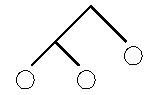
\includegraphics{img/tree1.pdf}\qquad\qquad
  \reflectbox{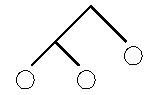
\includegraphics{img/tree1.pdf}}\quad\qquad
  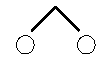
\includegraphics{img/tree2.pdf}
\end{center}
\caption{Containers de árbol}
\label{fig:Tree}
\end{figure}

La definición del conjunto de formas no difiere en mucho de la definición
inductiva del tipo \AgdaDatatype{Tree}.\footnote{Notar
  que lo mismo sucede con las listas. El conjunto de formas resulta
  ser el de los naturales, cuya definición tiene la misma estructura
  que la de las listas, sólo que ignorando los datos que se almacenan} 

\ExecuteMetaData[latex/Examples.tex]{treeSh}

Las posiciones posibles dependerán de las formas y serán tantas como
hojas haya. Por cada hoja hay una posición y para una forma \AgdaInductiveConstructor{nodeSh} $l\ r$, hay posiciones a la izquierda y a la derecha. 

\ExecuteMetaData[latex/Examples.tex]{treePos}

Finalmente, el container de los árboles binarios con datos en las hojas queda dado por:

\ExecuteMetaData[latex/Examples.tex]{ctree}


Observar que si quisiéramos representar árboles con la información almacenada en
los nodos, sólo cambiaríamos el conjunto de las posiciones, que dependerá de cuántos nodos tenga cada forma.

Otra cuestión interesante de destacar es el nivel de complejidad de notación que se alcanza al momento de representar árboles. En el capítulo \ref{chapter:construcciones} veremos que contamos con ciertos mecanismos de construcción de containers que proveen una suerte de modularidad, pudiendo componer containers de diversas maneras.
Estudiaremos allí un álgebra de containers.
\end{example}


\section{Morfismos de containers}

En esta sección presentaremos una forma de escribir funciones polimórficas entre tipos funtoriales. La estrategia a seguir es similar a la tomada en la sección anterior. Proveeremos una forma de definir conjuntos de códigos sintácticos, que habremos de llamar {\it morfismos de containers} y una función de extensión que los reinterprete.

Sean los containers
\AgdaFunction{cF}, \AgdaFunction{cG} \AgdaSymbol{:} \AgdaDatatype{Cont}
que representan a los constructores de tipos \AgdaDatatype{F}, \AgdaDatatype{G}  \AgdaSymbol{:} \AgdaDatatype{Set} \AgdaSymbol{$\to$} \AgdaDatatype{Set} respectivamente.
Es decir, \agdaExt{\AgdaFunction{cF}} $\cong$ \AgdaDatatype{F} y \agdaExt{\AgdaFunction{cG}} $\cong$ \AgdaDatatype{G}.

El objetivo es presentar una forma de representar ciertas funciones
\AgdaFunction{f} : \AgdaSymbol{$\forall$}\AgdaBound{$\{$X$\}\to$} \AgdaDatatype{F} \AgdaBound{X} \AgdaSymbol{$\to$} \AgdaDatatype{G} \AgdaBound{X}
como un morfismo de containers
\AgdaFunction{cf} : \AgdaFunction{cF} \AgdaFunction{$\Rightarrow$} \AgdaFunction{cG}.
En particular, nos interesan las \AgdaFunction{f} que 
preserven la estructura funtorial, es decir, que resulten ser {\it transformaciones naturales}.

\begin{definition} Sean los funtores \AgdaDatatype{F}, \AgdaDatatype{G}  \AgdaSymbol{:} \AgdaDatatype{Set} \AgdaSymbol{$\to$} \AgdaDatatype{Set}. Una función $f$ : \AgdaSymbol{$\forall$}\AgdaBound{$\{$X$\}\to$} \AgdaDatatype{F} \AgdaBound{X} \AgdaSymbol{$\to$} \AgdaDatatype{G} \AgdaBound{X} es una {\it transformación natural} si cumple, para toda $h : X \to Y$ y para alguna noción de igualdad.

\sangrar
\AgdaFunction{map} $h\ \circ$ $f$ = \AgdaFunction{f} $\circ$ \AgdaFunction{map} $h$

Notar que de cada lado de la igualdad, $f$ y \AgdaFunction{map} se instancian de forma diferente. Es decir, si agregamos los elementos implícitos como subíndices la ecuación de arriba nos queda: 

\sangrar
\AgdaFunction{map}$_{G}\ h\ \circ\ f_{X}$ = $f_{Y}\ \circ$ \AgdaFunction{map}$_{F}\ h$
\end{definition}

Para ello, definiremos un mecanismo de extensión que notaremos\ \agdaExtMorph{$\_$} tal que\\
\agdaExtMorph{\AgdaFunction{cf}} : \AgdaSymbol{$\forall$}\AgdaBound{$\{$X$\}\to$} \agdaExt{\AgdaFunction{cF}} \AgdaBound{X} \AgdaSymbol{$\to$} \agdaExt{\AgdaFunction{cG}} \AgdaBound{X}
y así obtener
\agdaExtMorph{\AgdaFunction{cf}} $\cong$ \AgdaFunction{f}. La función \agdaExtMorph{\AgdaFunction{cf}} resultante de extender el morfismo \AgdaFunction{cf} será una transformación natural entre los funtores container \agdaExt{\AgdaFunction{cF}} y \agdaExt{\AgdaFunction{cG}}.

\vspace{2ex}

Para comenzar la exposición analizaremos un ejemplo.
\begin{example}\label{ex:head}
Echemos un vistazo a la siguiente función, que retorna el primer elemento de una lista, si lo hay.

\ExecuteMetaData[latex/Aux.tex]{head}

Intuitivamente, un morfismo entre dos containers proveerá una forma de {\it reubicar} los elementos del primer container dentro del segundo.
¿Qué necesitamos proveer para crear una función \AgdaFunction{chead} que transforme un elemento de \AgdaFunction{cList} en uno de \AgdaFunction{cMaybe} de la forma esperada?
Por una lado necesitamos una función de \Sh \AgdaFunction{cList} en \Sh \AgdaFunction{cMaybe} para poder indicar que la lista vacía se transforma en el elemento \AgdaInductiveConstructor{nothing} y que para cualquier otra longitud de lista obtendremos la forma \AgdaInductiveConstructor{just} $\bigcirc$.  
Además necesitamos saber desde qué posiciones del container \AgdaFunction{cList} provienen los datos a guardar en el container imagen y así {\it reubicar} los valores almacenados. Para ello basta con dar una función que dada una posición de \AgdaFunction{cMaybe} nos indique una posición de \AgdaFunction{cList}, para cada forma.
En el caso de \AgdaFunction{head} habrá que indicar que el dato a guardar en la única posición de la forma \AgdaInductiveConstructor{just} $\bigcirc$ proviene de la primera posición de una lista de al menos un elemento, como muestra la figura \ref{fig:morph}.

\begin{figure}[H]
\begin{center}
  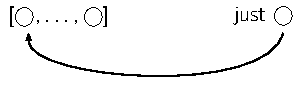
\includegraphics{img/morfismo2.pdf}
\end{center}
\caption{reubicando las posiciones según el comportamiento de \AgdaFunction{head}}
\label{fig:morph}
\end{figure}
\end{example}


\subsection{Definición y extensión de morfismos de container}

\begin{definition}
  Un {\it morfismo de containers} entre los containers $C_1$ y $C_2$ es un par de funciones $(m_{Sh}, m_{Pos})$, donde
  \begin{itemize}
    \item $m_{Sh}$ es una función que mapea las formas de $C_1$ hacia las formas de $C_2$
    \item Por cada forma $s$ de $C_1$, $m_{Pos}$ es una función que mapea cada posición de $C_2$ en la forma $m_{Sh}\ s$ hacia las posiciones de $C_1$ en la forma $s$.
  \end{itemize}
\end{definition}

Su formalización en Agda se expresa en el siguiente código:
\begin{agdacode}\label{code:morph}{\it Formalización de los morfismos de containers}

\ExecuteMetaData[latex/Container.tex]{morph}
\end{agdacode}

La componente \mSh del morfismo indica cómo transformar cada elemento del primer conjunto de formas en uno del segundo. La función \mPos es la encargada de reubicar los elementos a almacenar, indicando para cada posición del container imagen, una posición en el container origen.

\begin{definition} Sea $f$ un morfismo entre los containers $C$ y $D$. La {\it extensión} de $f$ sobre un conjunto $X$, que notamos \agdaExtMorph{$f$}, es una función entre los funtores containers \agdaExt{$C$} y \agdaExt{$D$} dada por el siguiente código:

\begin{agdacode}\label{code:morph:ext}{\it Extensión de morfismos de containers}

\ExecuteMetaData[latex/Container.tex]{morphExt}
\end{agdacode}

Al aplicar \agdaExtMorph{$f$} al elemento dado por una forma $c_s$ y una función $c_p$ de posiciones en valores, obtenemos otro container. Su forma la obtenemos gracias a la aplicación de la función de formas \mSh $f$. Dada una posición en esta nueva forma, \mPos $f$ indicará de dónde provienen los datos a guardar allí, información que completará la función $c_p$ .
\end{definition}

Un resultado muy interesante de esta construcción es que los morfismos de containers representan exactamente al conjunto de las transformaciones naturales entre los funtores \agdaExt{$C$} y \agdaExt{$D$}. Utilizando el universo de containers y morfismos nos aseguramos que las funciones definidas entre dos funtores containers serán transformaciones naturales, siendo imposible definir algo que no lo sea. Más aún, toda transformación natural $t$ entre \agdaExt{$C$} y \agdaExt{$D$} es representable en el universo de morfismos de containers por un elemento $f$, de forma tal que $\agdaExtMorph{$f$} = t$.

\begin{example} Para completar el ejemplo \ref{ex:head} expuesto en la introducción, veamos finalmente cómo queda definido el morfismo \AgdaFunction{chead}:

\ExecuteMetaData[latex/Examples.tex]{chead}

La función entre formas mapea la longitud de lista cero al elemento \AgdaInductiveConstructor{false}, representante del constructor \AgdaInductiveConstructor{nothing}. Para cualquier otra longitud de lista la forma resultante es \AgdaInductiveConstructor{true}, que indicaba la forma \AgdaInductiveConstructor{just}.

La función entre posiciones es vacía para el caso de las listas vacías puesto que allí no existen posiciones. En cualquier otra situación se mapea la posición única \AgdaInductiveConstructor{tt} a la primera de la lista. 

\ExecuteMetaData[latex/Examples.tex]{head}
\end{example}

\begin{definition}\label{code:morph:comp}Se define la {\it composición} entre dos morfismos de containers componiendo respectivamente las funciones de formas y posiciones, según se muestra en el siguiente código:
  
\ExecuteMetaData[latex/Container.tex]{morphComp}
\end{definition}

\begin{example}\label{code:morph:id}{\it Morfismos de containers identidad}

Dado cualquier container $C$, existe el morfismo identidad, que deja fija las formas y las posiciones.
  
  \ExecuteMetaData[latex/Container.tex]{morphId}
  Notar que la extensión de dicho morfismo será la función identidad.
\end{example}

\subsection{Equivalencia de morfismos}

Un lema que nos resultará muy útil para demostrar equivalencias en esta sección es aquél que prueba la igualdad de morfismos de containers. Dos morfismos de containers $f$ y $g$ son equivalentes siempre que lo sean sus componentes, las funciones de formas y posiciones.

\begin{agdacode}\label{morph:equivalence}{\it Equivalencia entre morfismos de containers}
  
\ExecuteMetaData[latex/Container.tex]{equivalence}
\end{agdacode}

Este es un claro ejemplo donde Agda no puede resolver trivialmente una equivalencia por no poder unificar los tipos de los argumentos.
Agda sólo nos permite probar por \AgdaInductiveConstructor{refl} una vez hecho pattern matching en los argumentos de \AgdaFunction{mEq}.
Esto es así puesto que sólo una vez probada la equivalencia de las funciones de formas, las funciones de posiciones tienen exactamente el mismo tipo.

Entonces, yendo paso a paso, el único habitante de \mSh $f$ \AgdaFunction{$\cong$} \mSh $g$ es \AgdaInductiveConstructor{refl}. Indicado esto, Agda unifica esta equivalencia y es posible hacer pattern matching en el segundo argumento. Al unificar la prueba de \mPos $f$ \AgdaFunction{$\cong$} \mPos $g$ la prueba final resulta trivial. 


\section{Categoría de containers}\label{cont:cat}

Dedicamos esta sección a presentar la formalización de los containers como una categoría. Los objetos de la categoría, que habremos de llamar $\Cont$ resultan ser los containers, definidos en \ref{code:cont}. El conjunto de morfismos será el de los morfismos de containers, expuesto en \ref{code:morph}. Como hemos mostrado en \ref{code:morph:comp} y \ref{code:morph:id}, los morfismos pueden componerse y siempre existe la identidad.

\begin{agdacode}\label{code:cont:cat}{\it Categoría de containers}

\ExecuteMetaData[latex/CatCont.tex]{cont}
\end{agdacode}
